\task{ В комнате на столе в патронах стоят 3~лампочки. Снаружи у 
двери комнаты имеются три выключателя, каждым из которых можно 
включить только одну лампочку. Определите каким ключом 
включается каждая лампочка, если открыть дверь и войти в комнату 
можно только один раз. Опишите свои действия. }

\task{ Тело подвешено на пружине динамометра.  При взвешивании тела 
в пустоте показания динамометра $P$.  При взвешивании этого же 
тела в жидкости с плотностью $\rho_1$ динамометр показывает $P_1$. При 
взвешивании тела в жидкости с неизвестной плотностью $\rho_2$ 
динамометр показывает $P_2$. Какова плотность жидкости $\rho_2$? При 
взвешивании тело полностью погружается в обе жидкости и не 
растворяется в них. }

\taskpic{ Груз весом $P$ подвешен на невесомом шарнире с тремя 
звеньями. Определите силу натяжения нити, соединяющей точки 
шарнира А и В. }{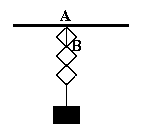
\includegraphics[width=3cm]{03.png}}

\task{ Сколько времени потребуется для превращения 2~л воды, взятой 
при температуре 20$^\circ$C в пар с температурой 100$^\circ$C? Нагревание 
происходит на горелке, расходующей 0{,}69~кг керосина в час. 
Теплоемкостью сосуда, в котором находится вода, пренебречь. 
Считать, что все тепло при сгорании керосина подводится к воде. 
Удельная теплота сгорания керосина $q = 4{,}6\cdot 10^7$~Дж/кг, удельная 
теплоемкость воды $c=4{,}2\cdot 10^3$~Дж/(кг$\cdot^\circ$C), удельная теплота 
парообразования воды $L=2{,}3\cdot10^6$~Дж/кг. }

\task{ Оцените массу атмосферы Венеры. Венеру считать шаром с 
площадью поверхности $4{,}7\cdot10^{14}$~м$^2$. Величина $g$ для Венеры равна 
  $8{,}7$~Н/кг. Атмосферное давление у поверхности Венеры 9120~кПа. }

\taskpic{ Два одинаковых проводника, изготовленных так, что их 
удельное сопротивление линейно изменяется с расстоянием от 
начала проводника: $\rho = kL$, где $\rho$ --- удельное сопротивление 
проводника, $k$ --- известный постоянный коэффициент,  $L$ --- 
расстояние от начала проводника до данной точки, соединены 
параллельно так, что у одного удельное сопротивление возрастает 
справа налево, а у другого наоборот --- слева направо. Эта схема 
подключена к источнику постоянного тока с напряжением $U_0$ 
(см.рис.). Какое напряжение показывает идеальный вольтметр, 
соединяющий середины этих проводников? }{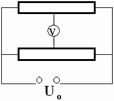
\includegraphics[width=2.5cm]{06.png}}

\task{ По прямому участку железнодорожного пути движется вагон со 
скоростью 14{,}4~км/ч. В вагоне мальчик пускает игрушечный состав по 
рельсам, расположенным поперек вагона. Скорость состава 
относительно пола вагона равна 3~м/с. Найти скорость игрушечного 
состава относительно Земли. }

\task{ Том вплотную подобрался к Джерри, двигаясь с постоянной 
скоростью $v$. В этот момент Джерри начинает убегать от Тома, 
двигаясь по прямой со скоростью $u$ = $k/R$, где $R$ --- расстояние между 
котом и мышью, $k$ --- постоянный независимый коэффициент. Найти 
установившееся расстояние между ними. }

\taskpic{ Из четырех нихромовых проволочек с удельным 
сопротивлением $\rho$, площадью сечения $S$, длиной $L$ каждая, 
выполнена фигура, представляющая собой крест. Крест подключают к 
источнику постоянного тока напряжением $U$, как показано на 
рисунке (положительный полюс к точке пересечения проволочек, 
отрицательный полюс к концам креста). Фигуру помещают в термос с 
дистиллированной водой. В некоторый момент времени  замыкают 
ключ. Вода закипела через время $\Delta t$. Сколько воды находилось в 
термосе? Удельная теплоемкость воды $c$, начальная температура $T$.  
Потерями тепла пренебречь. }{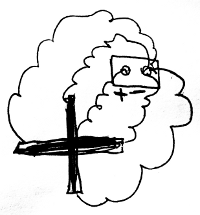
\includegraphics[width=4cm]{09.png}}

\taskpic{ По горизонтальной плоскости скользит без трения точечная 
шайба массы $m$. Скорость шайбы $v$. Перпендикулярно направлению 
движения шайбы движется лента транспортера с такой же по модулю 
скоростью $v$. Ширина транспортера $H$. Какой должна быть сила 
трения между поверхностями шайбы и транспортера для того, чтобы 
шайба переехала через него? }{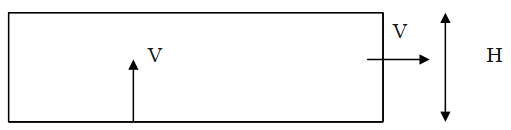
\includegraphics[width=4cm]{10.png}}

\task{ Три брата вместе выехали на конях из дворца и поехали к Кощею 
Бессмертному. Братья ехали по одной дороге, скорость каждого из 
них была постоянна. Скорость среднего брата равнялась 24~км/ч, 
скорость младшего брата --- 20~км/ч. Первым к Кощею приехал старший 
брат, спустя 1~час к Кощею приехал средний брат. Через 1~час после 
приезда среднего брата к Бессмертному приехал младший брат. 
Найдите скорость старшего брата. }

\task{ На горизонтальной шероховатой поверхности лежит цепочка из 
$N$ шариков массы $m$ каждый, связанных пружинками жесткости $k$. Все 
пружинки одинаковые и подчиняются закону Гука ($F_{\mbox{\textit{упр}}} = 
-kx$). Длина каждой пружинки в нерастянутом состоянии равна 0. 
Цепочку как-то растянули. Найдите максимально возможную длину 
цепочки, при которой все шарики неподвижны. Коэффициент трения 
между поверхностью и шариками равен $\mu$, ускорение свободного 
падения равно $g$. Размерами шариков пренебречь. }

\task{ Имеются две трубы, подсоединенные к смесителю. На каждой из 
труб имеется кран, которым можно регулировать поток воды по 
трубе, изменяя его от нуля до максимального значения~1 л/с. В 
трубах течет вода с температурами $t_1$ = 20$^\circ$C и $t_2$ = 60$^\circ$C. Из 
смесителя вытекает вода, температура которой во всех точках 
одинакова. Постройте график зависимости максимального потока 
воды, вытекающего из смесителя, от температуры этой воды. }

\task{ Два автомобиля находятся на шоссе на расстоянии 5~км друг от 
друга. По правилам гонки они обязаны все время двигаться с 
ускорением 1~м/с$^2$ относительно земли, причем направление 
ускорения каждый из них может менять в любой момент времени и 
неограниченное число раз. Гонка считается завершенной, когда 
автомобили оказываются рядом друг с другом и их скорости 
относительно друг друга в этот момент равны нулю. Найдите 
минимальное возможное время от начала гонки до ее завершения. }

\taskpic{ Две пружины с коэффициентами жесткости 12~Н/м и 8~Н/м  и легкая 
шайба, скользящая вдоль стержня без трения,  соединены вместе, 
как показано на рисунке. К свободному концу пружины прикладывают 
такую силу $F$, что он движется вправо с постоянной скоростью 
0{,}1~м/с. Найдите скорость шайбы. Постройте график зависимости 
прикладываемой силы $F$ от времени. }{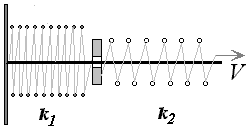
\includegraphics[width=4cm]{15.png}}

\taskpic{ Найдите наибольший объем легкой оболочки гелиевого 
метеорологического зонда, который может быть удержан невесомым 
нерастяжимым тросом, прикрепленным к двум одинаковым легким 
пластинам площадью 0{,}07~м$^2$, плотно притертым друг к другу. Нижняя 
пластина жестко прикреплена к земле. Плотность гелия равна 
0{,}178~кг/м$^3$, плотность воздуха --- 1{,}293~кг/м$^3$, атмосферное давление 
принять равным 10$^5$~Па. }{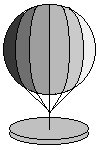
\includegraphics[width=2cm]{16.png}}

\task{ Из муравейника за гусеницей, расстояние до которой 1~м, 
выползает группа муравьев. Все муравьи движутся с постоянными 
скоростями, которые у разных особей разные и меняются от 1~см/с до 
2~см/с. Через 30~с муравей Ферда, который до этого двигался со 
скоростью 1~см/с, начинает двигаться с переменной скоростью, 
причем его скорость всегда в два раза выше, чем скорость 
окружающих его в данный момент муравьев. Успеет ли Ферда первым 
прибежать к гусенице?  Считайте, что характер движения других 
муравьев при этом не меняется. }

\task{ Отбросив с помощью зеркальца на близкую поверхность 
солнечный зайчик, наблюдатель затем расположил параллельно 
зеркальцу на малом расстоянии от него карандаш. Как при этом 
изменится вид солнечного зайчика? }

\task{ Два кота загнали мышку в узкий коридор и с двух сторон 
приближаются к ней, а мышка бегает между ними. Сколько раз мышка 
успеет добежать от одного кота до другого,  если скорость ее 
движения 2~м/с, а коты <<наступают>> со скоростью 0{,}5~м/с? Мышка 
поворачивает каждый раз на расстоянии 0{,}5~м от кота, не тратя на 
это времени. Мышка прекратит сопротивление, когда расстояние 
между котами будет равно 1{,}5~м. Известно, что длина коридора 10~м, 
коты начали двигаться одновременно и мышка в начальный момент 
была на расстоянии 0{,}5~м от одного из котов. }

\task{ Тело отпускают на высоте 15~м над стальной плитой. Удары тела о 
плиту абсолютно упругие. Постройте графики зависимости скорости 
тела и пути, пройденного телом, от времени за первые 6~секунд 
движения. }

\task{ В сосуде у поверхности воды плавает кусок льда с вмерзшей в 
него медной дробинкой массой 3~г. Сосуду сообщили 24~кДж теплоты, и 
дробинка утонула. Кусок льда какой массы плавал у поверхности?
Температура воды и льда 0$^\circ$С. Удельная теплота плавления льда 
$\lambda_{\mbox{\textit{в}}}$ = 340~кДж/кг, плотность воды $\rho_{\mbox{\textit{в}}}$ = 
1000~кг/м$^3$, плотность льда $\rho_{\mbox{\textit{л}}}$ = 900~кг/м$^3$, плотность 
меди $\rho_{\mbox{\textit{м}}}$ = 8900~кг/м$^3$. }

\task{ На какой глубине должна находиться опора, чтобы цилиндр 
высотой 24~см, плотно стоящий на ней, не всплывал? Плотность 
материала цилиндра в два раза меньше плотности воды, а площадь 
сечения в сто раз больше площади опоры. Атмосферное давление 
100~кПа, плотность воды 1000~кг/м$^3$. Соприкасающиеся поверхности 
цилиндра и опоры считать абсолютно гладкими. Ускорение 
свободного падения принять равным 10~м/с$^2$. }

\taskpic{ Двое друзей рассказывали, как здорово они умеют ездить на 
велосипеде. Первый говорит: <<Однажды я так сумел проехать, что 
график зависимости скорости от времени представлял точную 
полуокружность>>. <<А я умудрился так проехать, --- говорит другой, -- 
что этот график представлял равнобедренный треугольник>>. 
Определите, какое расстояние проехал каждый из них за 10~секунд, 
рассчитайте их средние скорости и определите, кто из них приврал. 
}{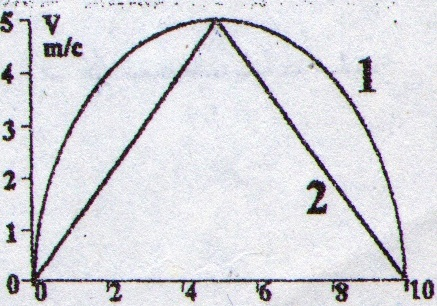
\includegraphics[width=4cm]{23.jpg}}

\task{ Во сколько раз будет отличаться минимальная начальная 
скорость, необходимая для того, чтобы перепрыгнуть яму, от 
минимальной начальной скорости, с которой можно перебраться 
через ту же яму с помощью жесткого легкого шеста, опирающегося на 
центр дна ямы? Глубина ямы $H$, ширина $L$. }

\task{ Горит башня, причем возгорание произошло в двух местах: 
первое --- на 1/10 высоты башни, а второе на $L$ = 220~м выше. Пламя 
распространяется вверх в 7 раз быстрее, чем вниз. Башня сгорела 
дотла за $t_1$ = 60~ч. Если бы $L$ было в 2~раза больше, башня бы сгорела 
за $t_2$ = 61~ч, а если бы в 2~раза меньше, то время бы не изменилось 
(60~ч). Чему была равна высота башни? }

\task{ Две дороги пересекаются под углом $\alpha$. По ним к перекрестку 
двигаются два автомобиля. Первый имеет скорость $v_1$, а второй --- 
$v_2$. В некоторый момент времени первый автомобиль находится на 
расстоянии $L_1$ от перекрестка, а второй на расстоянии $L_2$ от 
перекрестка. Найдите минимальное расстояние между автомобилями 
в процессе их движения. }

\taskpic{ Грузы, имеющие массы $M$ и $m$ ($M > m$), при помощи невесомой 
нерастяжимой нити подвешены на блоке. С каким минимальным 
ускорением нужно двигать блок в вертикальном направлении, чтобы 
ускорения грузов были направлены в одну сторону? Ускорение 
свободного падения $g$. Сопротивлением воздуха пренебречь. 
}{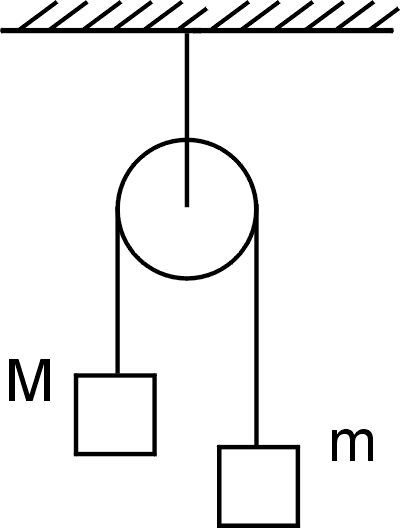
\includegraphics[width=2.5cm]{27.png}}

\task{ Катушку радиуса $R$, находящуюся на горизонтальной 
поверхности, тянут за нить, намотанную на ось катушки радиуса $r$. 
Нить движется со скоростью $v$ в горизонтальном направлении. 
Найдите поступательную скорость оси катушки относительно 
поверхности. Катушка не проскальзывает по поверхности. }

\task{ С помощью термометра измеряют попеременно температуры 
жидкостей, налитых в два калориметра. Показания термометра: 80, 16, 
78, 19 $^\circ$C. Что покажет термометр после следующего переноса? После 
большого числа переносов? }

\task{ Толстостенная лодка с вертикальными стенками и отверстием в 
дне достаточно долго свободно плавает в озере. Затем отверстие 
снаружи затыкают, и потом внутрь лодки пускают плавать бревно. 
Повысится или понизится после этого уровень воды в лодке 
относительно уровня воды в озере? }

\task{ В стакан с водой опустили нагреватель и сняли зависимость 
температуры воды $T$ от времени $t$ (см. таблицу). На сколько 
градусов остынет вода за 1~мин, если нагреватель отключили от 
сети при температуре 50$^\circ$C? Закипит ли вода, если нагреватель не 
выключать достаточно долго? Мощность нагревателя считать 
неизменной.

\begin{tabular}{| c | c | c | c | c | c | c | c | c | c | c |}
\hline
$t$,~мин & 0 & 1 & 2 & 3 & 4 & 5 & 6 & 7 & 8 & 9 \\
\hline
$T$,~$^\circ$C & 20 & 26,2 & 31,8 & 36,8 & 41,4 & 45,6 & 49,3 & 52,7 & 55,8 & 61,1 \\
\hline
\end{tabular} }

\task{ Вес $P$ системы, состоящей из стакана с водой и пробкового 
шарика, измеряют в следующих пяти случаях:
\begin{enumerate}
\item шарик свободно плавает в стакане (показания весов $P_1$);
\item шарик лежит на чашке весов рядом со стаканом ($P_2$);
\item шарик удерживается в полностью погруженном состоянии тонкой 
невесомой нитью, прикрепленной к дну стакана ($P_3$);
\item шарик удерживается в полностью погруженном состоянии тонкой 
невесомой спицей, закрепленной над стаканом ($P_4$);
\item шарик свободно всплывает ($P_5$).
\end{enumerate}
Расставить показания весов в порядке их возрастания. }

\task{ Две невесомые пружины имеют длины $l_1$, $l_2$ и жесткости $k_1$, $k_2$ 
соответственно. Одна пружина вставлена в другую. Концы пружин 
попарно скреплены. Другими точками пружины друг друга не 
касаются. Какова жесткость получившейся пружины? }

\task{ Моток голой проволоки, содержащей семь с половиной витков, 
растянут на двух вбитых в доску гвоздях, к которым присоединены 
его концы. Подключив к гвоздям приборы, измерили сопротивление 
цепи между гвоздями. Во сколько раз изменится это сопротивление, 
если моток снять с доски и размотать, оставив концы 
присоединенными к гвоздям? }

\task{ На поверхности озера Байкал зимой намерзает толстый слой 
льда. Предположим, что где-то в декабре толщина льда составляет $x$ 
= 80~см. Температура воздуха $t$ = 40$^\circ$С. С какой скоростью (в~мм/ч) 
увеличивается в этот период толщина слоя льда?

Для льда: плотность $\rho$ = 0{,}92~г/см$^3$, удельная теплота плавления 
$\lambda = 3{,}3\cdot10^5$~Дж/кг, коэффициент теплопроводности $k$ = 2{,}2 
Вт/(м$\cdot^\circ$C).

Количество теплоты, проходящее в единицу времени через слой 
вещества площадью $S$ и толщиной $h$ при разности температур $\Delta t$ 
между поверхностями, определяется соотношением $q = kS\Delta t/h$. }

\task{ Цилиндрический медный проводник площадью поперечного 
сечения $S$ = 0{,}1~см$^2$ подключается к источнику постоянного тока. 
Температура проводника начинает увеличиваться. Как видно из 
графика зависимости температуры от времени, через время $\tau_1$ = 
10~мин температура проводника становится равной $t_1$ = 90$^\circ$C.
\begin{enumerate}
\item За какое время температура проводника достигла бы значения 
$t_1$, если бы проводник был окружен теплонепроницаемой оболочкой?
\item Найдите силу тока в проводнике.
\item Предположим, что по истечении времени $\tau_2$ = 5~мин проводник 
был отключен от источника тока и начал остывать. Определите, за 
какое приблизительно время $\Delta\tau$ температура проводника 
изменится от 70$^\circ$C до 65$^\circ$C.
\end{enumerate}
Для меди: удельная теплоемкость $c$ = 390~Дж/(кг$\cdot^\circ$C), удельное 
сопротивление $\rho_{\mbox{\textit{м}}}$ = 1{,}75$\cdot 10^{-8}$~Ом$\cdot$м, плотность $\rho$ 
= 8{,}9$\cdot10^3$~кг/м$^3$. }
\begin{center}
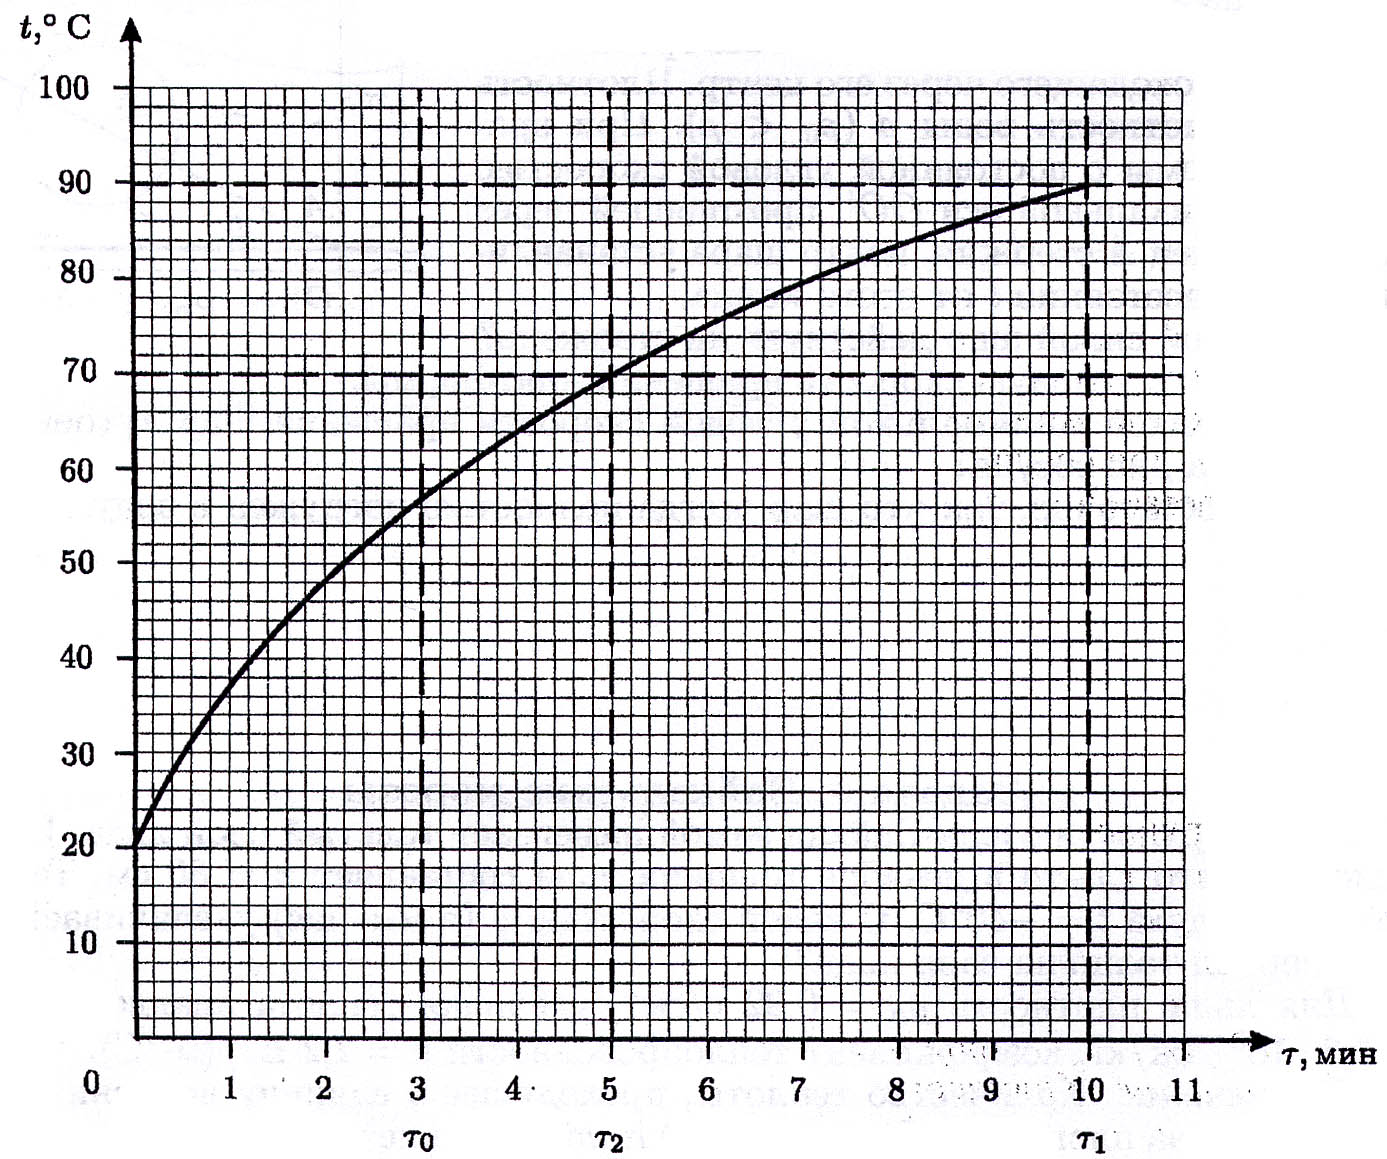
\includegraphics[width=12cm]{36.jpg}
\end{center}
